\chapter{初段ミューオントリガーの性能評価}
本章では、\ref{chapter4}で述べた手法で作成した2種類の CW (シミュレーション用の CW と実際の測定用の CW) を用いたトリガーの性能の評価を行う。
便宜上、本手法で作成した 2 種類の CW について、シミュレーション用の CW を $\mathrm{CW_{Simu}}$、実際の測定用の CW を $\mathrm{CW_{Data}}$ と呼び、2022年 Run-3 で使用された CW を $\mathrm{CW_{2022}}$ と定義する。

\section{機械学習で作成した CW を用いたトリガーの性能評価}
\subsection{評価方法}
式\ref{equ:Eff5}を用いて、全オフライン再構成されたミューオンの内、ある $p_T$ 閾値以上のトリガーが発行された割合 $\epsilon$ を計算し、トリガー効率の算出を行った。また、$\epsilon$ をオフライン再構成した $p_T$ の関数として表した Turn-on curve を描き、式\eqref{equ:fitting5} の関数によってフィッティングを行う事で、トリガー性能の評価を行った。
\begin{equation}
    \epsilon = \frac{ある p_T 閾値以上のトリガーを発行したミューオンの数}{全オフライン再構成したミューオンの数}
 \label{equ:Eff5}
\end{equation}
\begin{equation}
    f(p_T) = \frac{p_0}{exp(\frac{p_T-p_1}{p_2})+1}
 \label{equ:fitting5}
\end{equation}
ここで\ref{section:fitting}節で述べたように、$p_0$は Plateau efficiency、$p_1$は Effective threshold、$p_2$は Resolution を表している。

\subsection{機械学習を用いて作成した CW の 15 段階 $p_T$ 閾値}
Run-3 に向けて新たに作成した CW のトリガー効率の評価を行う。

$\mathrm{CW_{Data}}$ の図\ref{fig:15Eff_CW_Simu} に $\mathrm{CW_{Simu}}$ を用いて3 ステーションコインシデンスのみで hotroi フラグを要求した結果の15段階の $p_T$ 閾値における Turn-on curve を示す。$\mathrm{CW_{Simu}}$ の評価にはシングルミューオンのシミュレーションデータを用いた。
図\ref{fig:15Eff_CW_Data}に$\mathrm{CW_{Data}}$を用いて3 ステーションコインシデンスのみで hotroi フラグを要求した結果の15段階の $p_T$ 閾値における Turn-on curve を示す。評価には2018 年 Run-2 のデータに対して $Z \rightarrow \mu\mu$ による Tag $\&$ Probe 法を用いた。比較のため、図\ref{fig:Run3_15_MC5} に $\mathrm{CW_{2022}}$ の Turn-on curve を示す。

まず、2018年 Run-2 データを用いて本手法で作成した $\mathrm{CW_{Data}}$ と $\mathrm{CW_{Simu}}$ の比較を行う。図\ref{fig:v06v07}に同じ閾値の Turn-on curve を比較したプロットを示す。$\mathrm{CW_{Data}}$ の方が実際のデータに対してのトリガー効率が良くなっているのが見て取れる。これは、実際のデータを学習に使用したことで、検出器のズレに対応し、CW の最適化ができたことを示している。
\begin{figure}[tb]
  \centering
  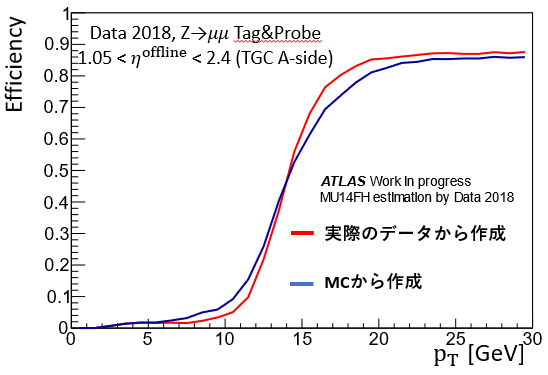
\includegraphics[clip, width=12cm]{fig/4/hikaku_v06_v07.png}
  \caption{v06v07}
  \label{fig:v06v07}
\end{figure}

次に、本手法で作成した $\mathrm{CW_{Data}}$ と $\mathrm{CW_{Simu}}$ を $\mathrm{CW_{2022}}$ と比較する。
図\ref{fig:v05v06} には $\mathrm{CW_{2022}}$ の各閾値と同程度のパフォーマンスでとなる $\mathrm{CW_{Simu}}$ の Turn-on curve を示し、図\ref{fig:v05v07} には $\mathrm{CW_{2022}}$ の各閾値と同程度のパフォーマンスでとなる $\mathrm{CW_{Data}}$ の Turn-on curve を示した。
各 Turn-on curve に\eqref{equ:fitting5}によるフィッティングを行い Turn-on curve の Resolitionvを比較する。図\ref{fig:Resolution_v07v05}に $\mathrm{CW_{Simu}}$ と $\mathrm{CW_{2022}}$ の比較、 図\ref{fig:Resolution_v06v05}に $\mathrm{CW_{Simu}}$ と $\mathrm{CW_{2022}}$ の比較を示す。
$\mathrm{CW_{2022}}$ よりも Resolution が良くなっていることが見て取れる。


\begin{figure}[tb]
  \centering
  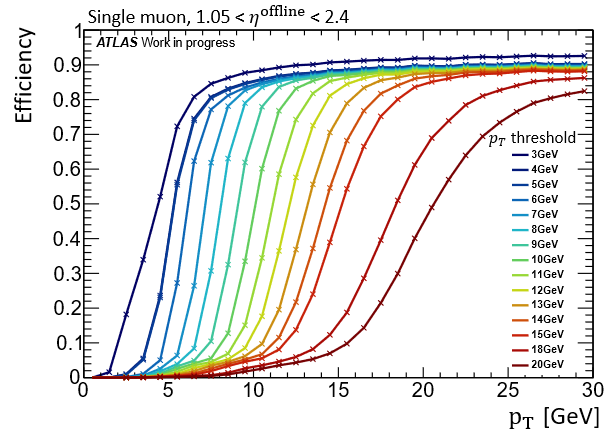
\includegraphics[clip, width=12cm]{fig/4/v07_15_Eff.png}
  \caption{<差し替え>シミュレーションデータをトレーニングに使用した機械学習を用いて作成した CW の 15 段階の閾値における Turn-on curve。}
  \label{fig:15Eff_CW_Simu}
\end{figure}

\begin{figure}[tb]
  \centering
  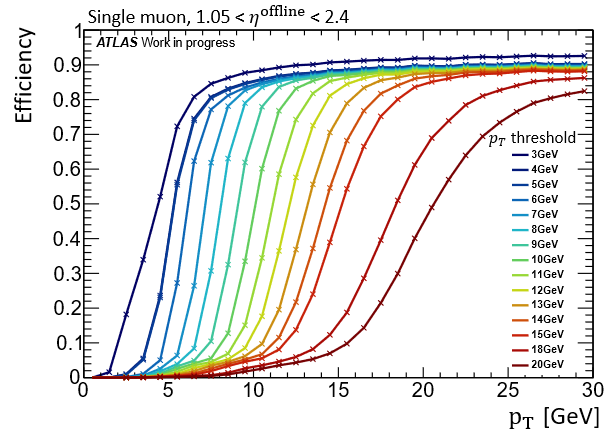
\includegraphics[clip, width=12cm]{fig/4/v07_15_Eff.png}
  \caption{<差し替え>2018年 Run-2 のデータをトレーニングに使用した機械学習を用いて作成した CW の 15 段階の閾値における Turn-on curve。}
  \label{fig:15Eff_CW_Data}
\end{figure}

\begin{figure}[tb]
  \centering
  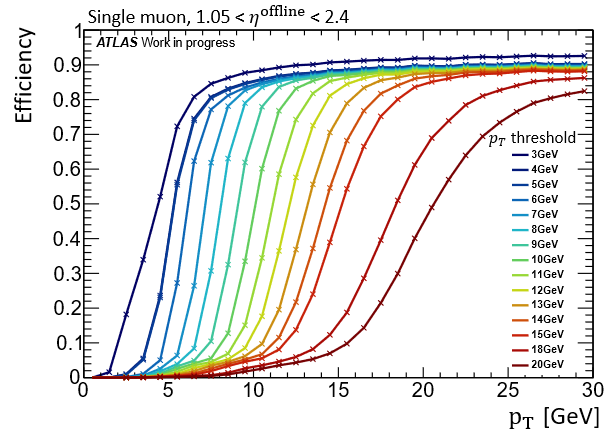
\includegraphics[clip, width=12cm]{fig/4/v07_15_Eff.png}
  \caption{<差し替え>2018年 Run-2 のデータをトレーニングに使用した機械学習を用いて作成した CW の 15 段階の閾値における Turn-on curve。}
  \label{fig:15Eff_CW_Data}
\end{figure}

\begin{figure}[tb]
  \centering
  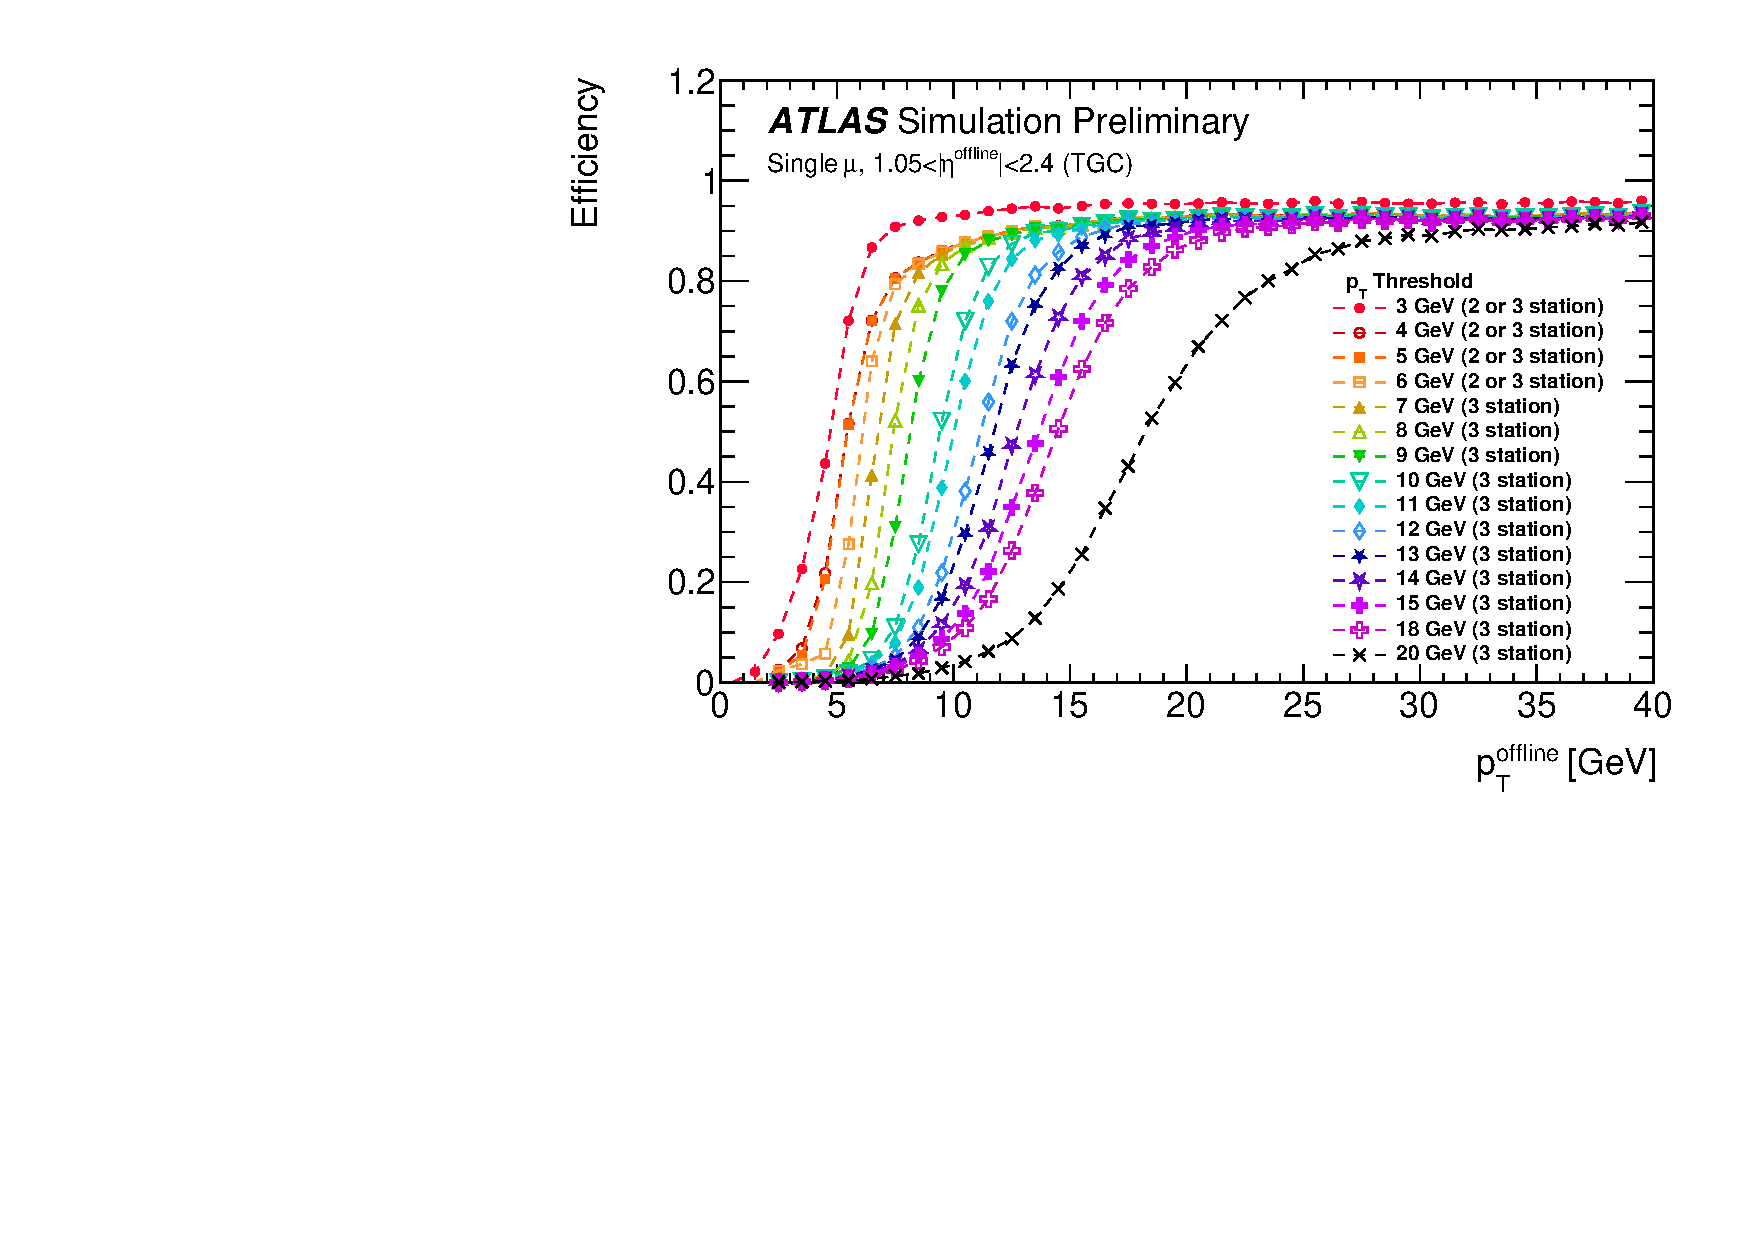
\includegraphics[clip, width=12cm]{fig/3/PLOT-TRIG-2020-01-fig1.pdf}
  \caption{Run-3 における15段階閾値のTurn-on curve。シングルミューオンのシミュレーションサンプルに対してのトリガー効率を示している。}
  \label{fig:Run3_15_MC5}
\end{figure}

\begin{figure}[tb]
  \centering
  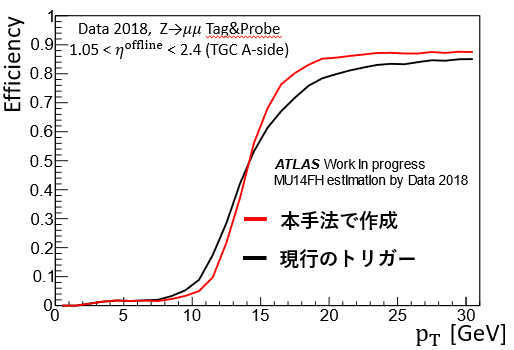
\includegraphics[clip, width=12cm]{fig/4/hikaku_v05_v06.png}
  \caption{v05v06}
  \label{fig:v05v06}
\end{figure}

\begin{figure}[tb]
  \centering
  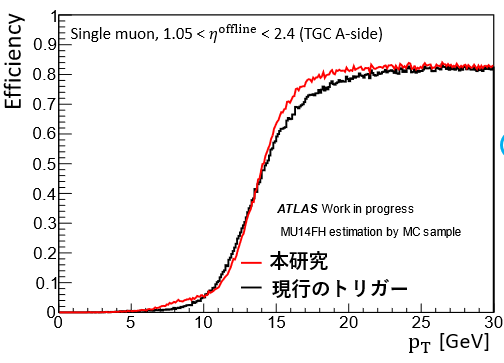
\includegraphics[clip, width=12cm]{fig/4/hikaku_v05_v07.png}
  \caption{v05v07}
  \label{fig:v05v07}
\end{figure}

\begin{figure}[tb]
  \centering
  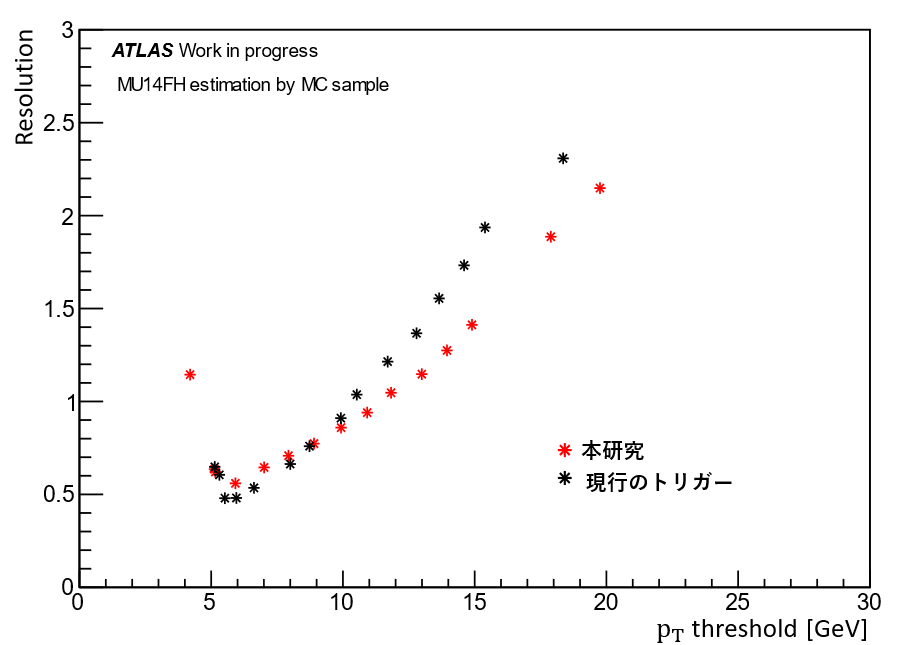
\includegraphics[clip, width=12cm]{fig/4/resolution_v07_v05.png}
  \caption{Resolutionv07v05}
  \label{fig:Resolution_v07v05}
\end{figure}

\begin{figure}[tb]
  \centering
  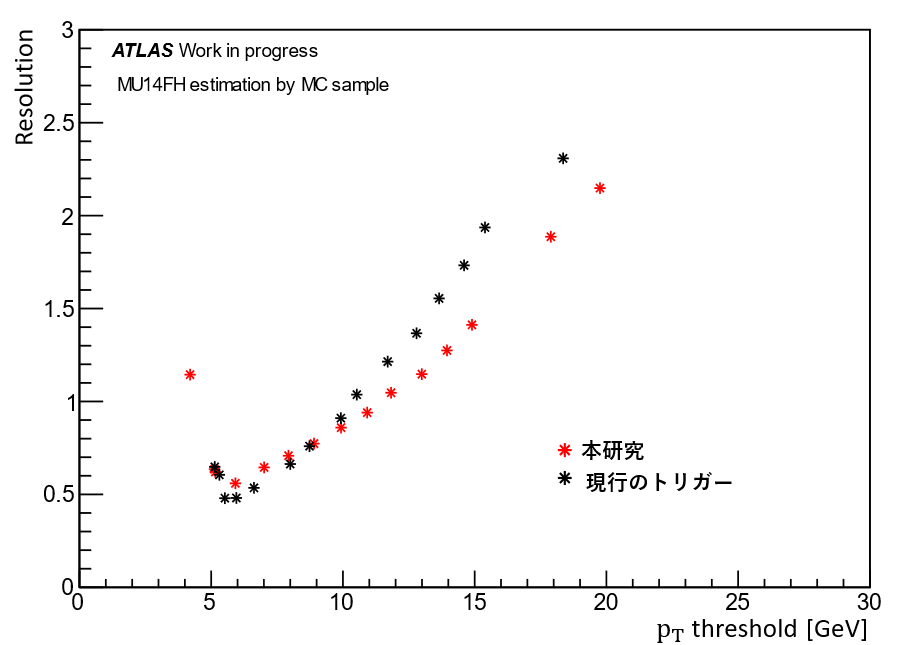
\includegraphics[clip, width=12cm]{fig/4/resolution_v07_v05.png}
  \caption{Resolutionv06v05}
  \label{fig:Resolution_v06v05}
\end{figure}

\subsection{ミューオン電荷に対するトリガー性能の評価}



\section{機械学習を用いることによる CW 作成の効果}
\subsubsection{チェンバーごとのEfficiency}
\begin{figure}[tb]
  \centering
  \rule{8cm}{6cm}
  %\includegraphics[clip, width=14cm]{}
  \caption{チェンバーごとのEfficiency (1-48)}
  \label{fig:fit_def}
\end{figure}

\subsubsection{ミューオンの電荷に対する効果}

\begin{figure}[tb]
  \centering
  \rule{8cm}{6cm}
  %\includegraphics[clip, width=14cm]{}
  \caption{Rate}
  \label{fig:fit_def}
\end{figure}


\section{Run-3に向けた本手法のトリガー性能}
Date と MC でeffの比較
\begin{figure}[tb]
  \centering
  \rule{8cm}{6cm}
  \caption{Efficiency}
  \label{fig:fit_def}
\end{figure}

\subsection{トリガーレート}
Date と MC
\begin{figure}[tb]
  \centering
  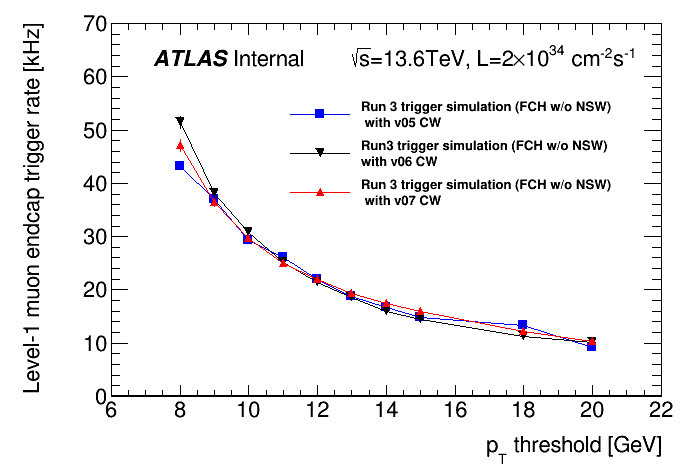
\includegraphics[clip, width=14cm]{fig/5/l1mue_rate_run3.png}
  \caption{Rate}
  \label{fig:fit_def}
\end{figure}


<TriggerRate>
\begin{figure}[tb]
  \centering
  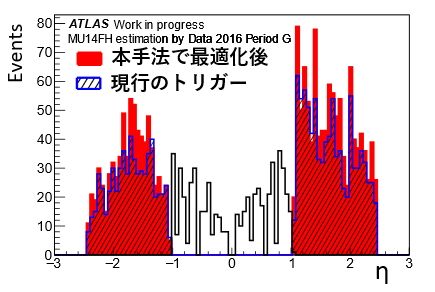
\includegraphics[clip, width=12cm]{fig/4/rate_v05_v06.png}
  \caption{v05v06}
  \label{fig:Resolution}
\end{figure}


